\begin{frame}{Процессы в UNIX}
  \begin{itemize}
    \item Создание процессов
      \begin{itemize}
        \item fork
        \item exec
      \end{itemize}
    \item Атрибуты процесса
      \begin{itemize}
        \item pid 
        \item файловые дескрипторы
        \item environment
        \item Рабочая директория (cwd)
        \item прочее в директории {\tt /proc/<pid>}
      \end{itemize}
  \end{itemize}
\end{frame}

\begin{frame}{Управление процессами}
  \begin{itemize}
    \item kill (killall)
    \item top
    \item pstree
    \item Команды управления процессами в bash: 
      \begin{itemize}
        \item {\tt jobs}, {\tt fg, \tt bg}
        \item Ctrl-C -- оборвать выполнение процесса (SIGINT)
        \item Ctrl-Z -- остановить выполнение команды (SIGTSTP)
        \item Ctrl-D -- завершить ввод
      \end{itemize}
  \end{itemize}
\end{frame}


\begin{frame}{Упражнения}
  \begin{block}{Посмотреть вывод pstree}
    {\tt pstree}
  \end{block}
  \pause
  \begin{block}{Ctrl-C, Ctrl-Z}
    В графическом режиме запустить из терминала emacs

    Ctrl-Z

    jobs -l

    bg +
  \end{block}
  \pause
  \begin{block}{fork bomb}

    {\tt ulimit -u 200} 

    {\tt bomb()\{ (bomb; bomb) \& \} }

    top

    killall bash

  \end{block}
\end{frame}


\begin{frame}{Unix way}
  \begin{enumerate}
    \item Пишите программы, которые делают одну вещь и делают её хорошо.
    \item Пишите программы, которые бы работали вместе.
    \item Пишите программы, которые бы поддерживали текстовые потоки, поскольку это универсальный интерфейс. 
  \end{enumerate}
\end{frame}

\begin{frame}{Unix way}
  \begin{enumerate}
    \item   Маленькое прекрасно.
    \item   Пусть каждая программа делает одну вещь, но хорошо.
    \item   Собирайте прототип как можно раньше.
    \item   Предпочитайте переносимость эффективности.
    \item   Храните данные в простых текстовых файлах.
    \item   Используйте программные рычаги для достижения цели.
    \item   Используйте сценарии командной строки для улучшения функционала и переносимости.
    \item   Избегайте <<связывающего>> (captive) пользовательского интерфейса.
    \item   Делайте каждую программу «фильтром».
  \end{enumerate}
\end{frame}

\begin{frame}{Конвееры}
%  \textbf{Цель} -- максимальная модульность: большое количество простых приложений, взаимодействующих друг с другом для решения задач
  \only<1>{
  \begin{center}
    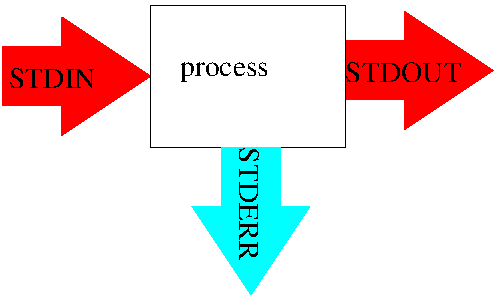
\includegraphics[width=1.2in]{../../slides/cmdline/process}
  \end{center}
  }
  \only<2>{
    \begin{center}
      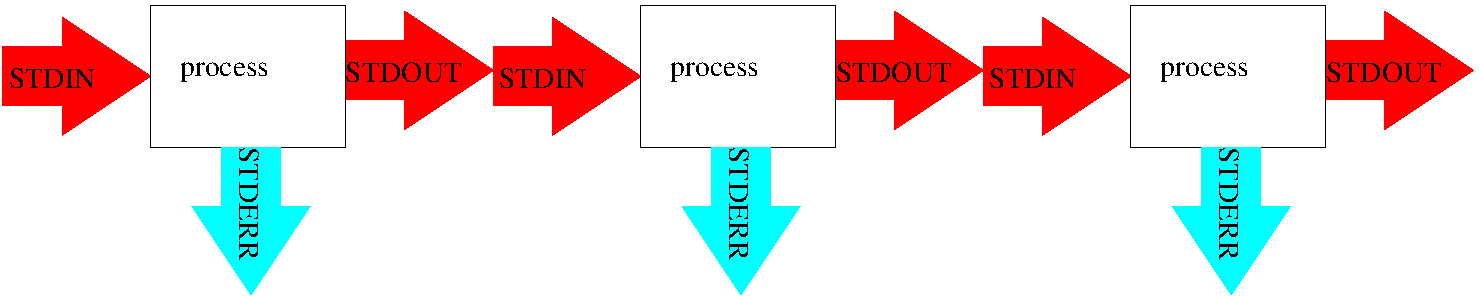
\includegraphics[width=3.6in]{../../slides/cmdline/processes}
    \end{center}
  }
  \begin{itemize}
    \item <1-> Каждое приложение открывает 3 стандартных файловых дескриптора stdin (fd 0), stdout(fd 1), stderr (fd 2)
    \item <2-> Приложения могут работать как фильтр из STDIN в STDOUT, можно объединять несколько приложений в конвейер
    \item <2-> Синтаксис {\tt <app1> | <app2>}
  \end{itemize}
\end{frame}
